\documentclass[11pt]{IEEEtran}
% \documentclass[11pt]{article}

\usepackage{blindtext}
\usepackage[colorlinks]{hyperref}
\usepackage{breakurl}
\usepackage{listings}
\usepackage[table,xcdraw]{xcolor}
\usepackage{fancyvrb}
\usepackage{graphicx}
\usepackage{float}
\usepackage{caption}
\usepackage{mathtools}

\newcommand{\nosection}[1]{\vspace{3pt}\noindent\textbf{#1}}
\newcommand{\fyi}[1]{\textcolor{blue}{#1}}
\def\eg{\textit{e.g.,}\hspace{1mm}}
\def\etc{\textit{etc.}\hspace{1mm}}
\newcommand{\secref}[1]{Sec.~\ref{#1}}
\newcommand{\figref}[1]{Fig.~\ref{#1}}
\newcommand{\tabref}[1]{Tab.~\ref{#1}}
\newcommand{\eqnref}[1]{Eqn.~\ref{#1}}

\definecolor{codegreen}{rgb}{0,0.6,0}
\definecolor{codegray}{rgb}{0.5,0.5,0.5}
\definecolor{codepurple}{rgb}{0.58,0,0.82}
\definecolor{backcolour}{rgb}{0.95,0.95,0.92}

\lstdefinestyle{mystyle}{
	% backgroundcolor=\color{backcolour},   
	commentstyle=\color{codegray},
	keywordstyle=\bfseries,
	numberstyle=\tiny\color{codegray},
	stringstyle=\color{codepurple},
	basicstyle=\ttfamily\scriptsize,
	breakatwhitespace=false,         
	breaklines=true,                 
	captionpos=b,                    
	keepspaces=true,                 
	% numbers=left,                    
	numbersep=5pt,                  
	showspaces=false,                
	showstringspaces=false,
	showtabs=false,                  
	tabsize=4,
	%frame=shadowbox,
	frame=l,
}

\lstset{linewidth=\linewidth}
\lstset{style=mystyle}

\newcommand{\sys}{\textsc{YeahCuckoo}\xspace}

\title{\sys: Improving Load Factor Using a Two-Dimensional Vector Space}
\author{Author: Chengke Wang \\
Student ID: 2101111452 \\ 
Email: chengke@pku.edu.cn}

\begin{document}
\maketitle

\section{Introduction}

Cuckoo filter \cite{cuckoo} can replace Bloom filter \cite{bloom} for approximate set membership tests. It has the advantages of support to add and remove items dynamically while preserving a low false positive rate. There are two fundamental insights behind such a filter design. First, Cuckoo use the power-of-two of Cuckoo hashing, enabling item online insertion and deletion. Second, it leverages the XOR operation with fingerprint hashing to ensure conflicted items can be relocated to an entirely different part of the hash bucket, therefore retaining a low hash collision and improving the data structure utilization. 

In this work we propose \sys, a variant of Cuckoo filter which improve the load factor. The key idea is that we use a K-dimensional vector space to kick items when the hash bucket is full. This idea derives from the aforementioned two insights in Cuckoo filter. First, the power-of-two allows an item placement at two buckets. If we can place the item at more than two buckets, we can achieve a higher load factor. Second, the XOR operation is a module-like algebraic structure. In fact, the Cuckoo filter use a 1-dimensional vector space to locate the bucket. Theoretically, we can extend it to K-dimensional, allowing a item to be placed at more different buckets.

We carry out experiment to show the \sys performance. The results indicates that, with a typical setting where there are 4 entries in a bucket and 12-bit fingerprints, \sys improves the load factor of 1.5\% at the cost of only 0.18\% increased false positive rate.

\nosection{Contributions}
\begin{itemize}
	\item We introduce \sys, a Cuckoo-variant algorithm that uses the XOR property to achieve higher load factor than vanilla Cuckoo filter. 
	\item We conduct an experiment showing that our design only increase the false positive rate of 0.18\%.
	\item We open source our implementation, which is available at GitHub \cite{yeah}.
\end{itemize}

\section{\sys Design}

\begin{figure}
\centering
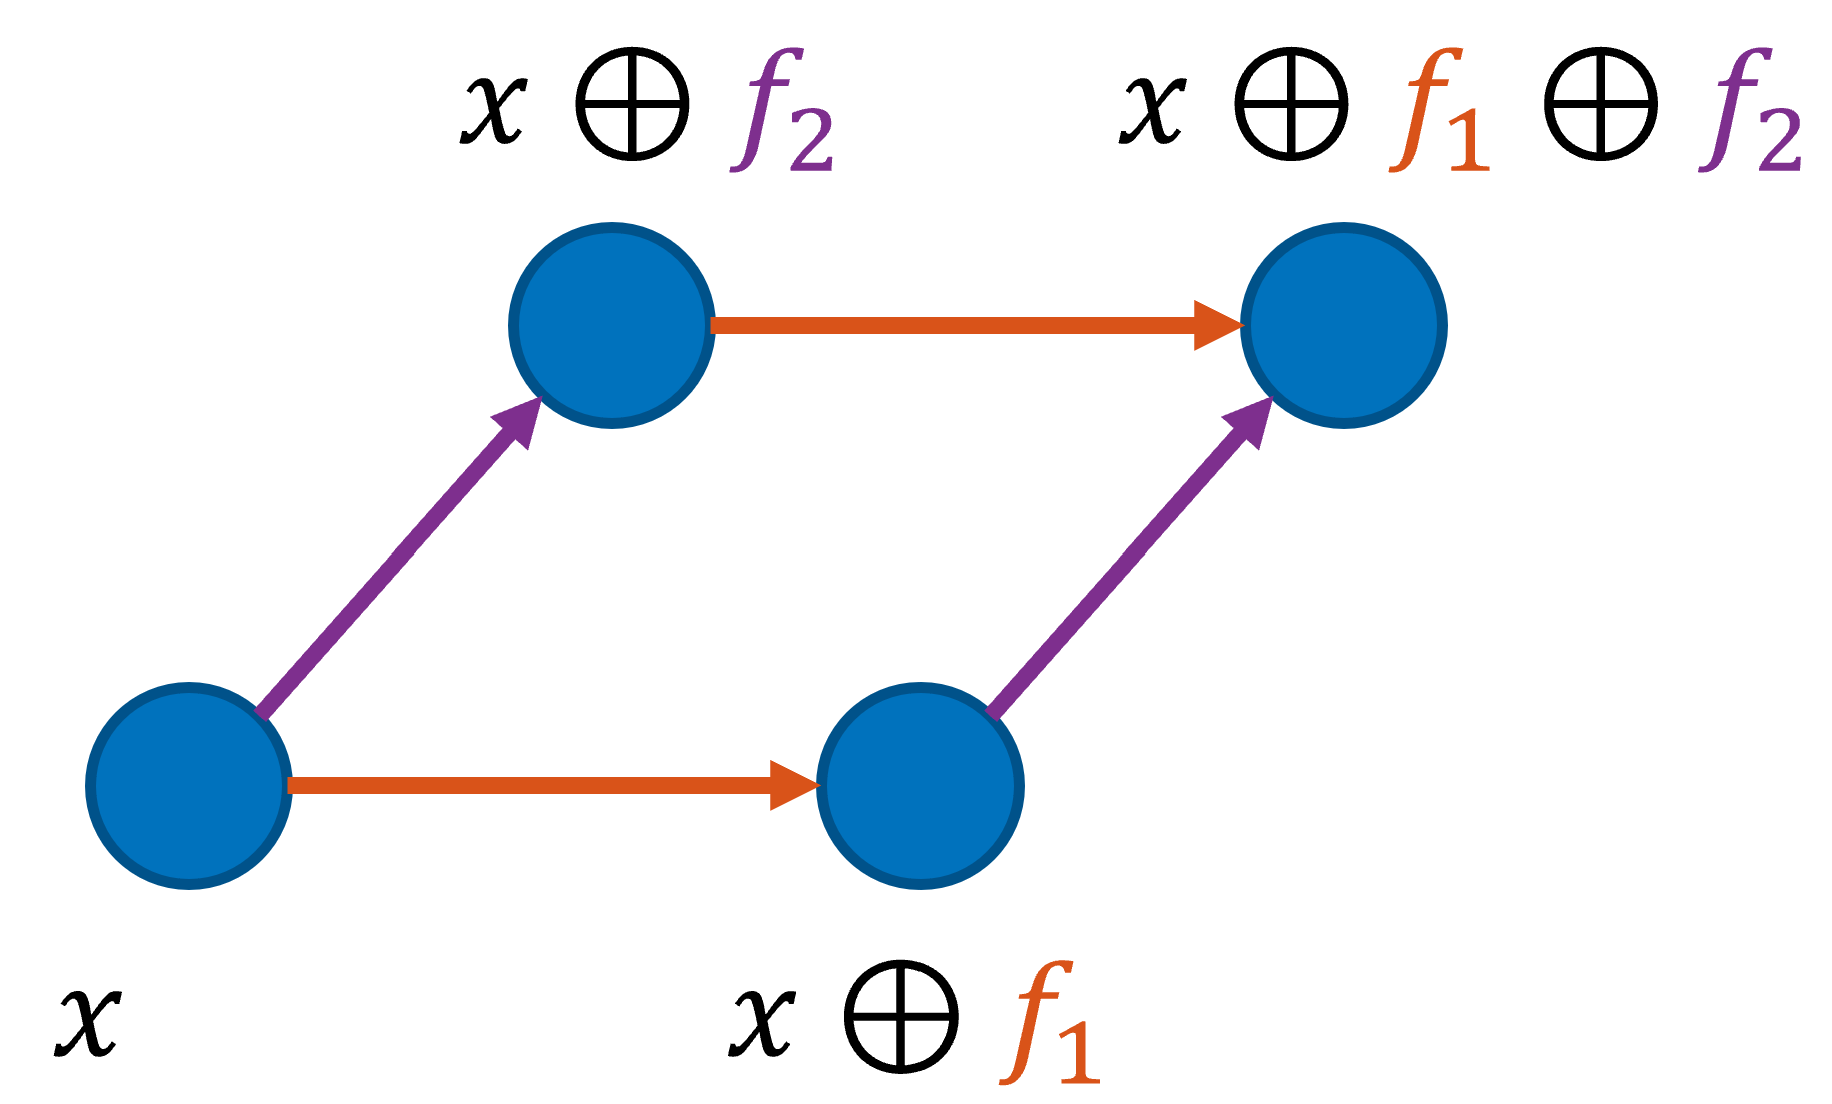
\includegraphics[width=0.6\linewidth]{design.png}
\caption{\sys uses a 2-dimensional vector space to locate buckets. The $f_1,f_2$ are two fingerprint hashes of item $x$.}
\label{design}
\end{figure}

We first recall how Cuckoo filter uses the XOR operation and then explain our design. 

Unlike Bloom filter, Cuckoo filter only stores fingerprints and therefore there is no way to restore and rehash the original keys from its location $i$ to find their alternate locations $j$. To address this problem, Cuckoo filter utilize a technique called partial-key cuckoo hashing to derive an item $x$'s alternate location based on its fingerprint. Let $\text{fp}(x)$ be the fingerprint of $x$. The key idea can be illustrated as:

\begin{equation*}
\begin{split}
i =& h_1(x) = \text{hash}(x) \\
j =& h_2(x) = h_1(x) \oplus \text{hash}(\text{fp}(x))
\end{split}
\end{equation*}

\sys follows this idea and extend this operation to 2-dimensional vector space. It can address three alternate locations $j, k, l$ other than location $i$. Therefore an item has double number of buckets to place and we can increase the load factor. Specifically, each hash of fingerprint create a simple algebraic space with two possible values. If we has two fingerprint hashes and perform a Cartesian product on them, we get a 2-dimensional vector space. The Figure~\ref{design} illustrates this. Formally, we have:

\begin{equation*}
\begin{split}
i =& h_1(x) = \text{hash}(x) \\
j =& h_2(x) = h_1(x) \oplus \text{hash1}(\text{fp}(x))\\
k =& h_3(x) = h_1(x) \oplus \text{hash2}(\text{fp}(x)) \\
k =& h_4(x) = h_1(x) \oplus \text{hash1}(\text{fp}(x)) \oplus \text{hash2}(\text{fp}(x))
\end{split}
\end{equation*}

For example, if $h_1(x)$ is 00 and two fingerprint hashes are $11$ and $10$, the item $x$ can be placed at bucket $00, 01,10$ and $11$. 

Note that \sys differs from the design where we just increase the number of entries per bucket because (1) To keep the same capacity, the number of buckets need to decrease. Therefore, hash collisions become more frequent. (2) Since there are more entries in the bucket, we need more time cost to iterate over the bucket. Our evaluation shows that \sys outperforms such design.

\section{Evaluation}

\subsection{Implementation and Setup}

We implement \sys with about 800 lines in C++ language. The code is available at GitHub~\cite{yeah}. To make the comparison, we also implement a vanilla Cuckoo filter. To reduce the run-time overhead, we leverage the template programming technique in C++, fixing the variables like the \verb|bits_per_fingerprint| at compile-time. We use CityHash~\cite{cityhash} as the hash function. The 64-bit hash result is used for generate bucket index and the XOR values. We use the Mersenne Twister with default parameters to generate items for insertion. To make the experiment reproducible, we fix the random seed. 

\subsection{Evaluation Results}

\bibliographystyle{IEEEtran} 
\bibliography{refs} 

\end{document}
